\begin{customAppendixPage}{Component Layout}
This section contains the diagrams of the designed Printed Circuit Boards.  In the diagrams shown, the component placement can be seen.  The reference numbers displayed on the PCB layout are the same that are found in the first and second level schematics that accompany the boards.

Recall that the PCB was designed with two levels.  Figure~\ref{fig:1stLvlSchem} and~\ref{fig:1stLvlBoard} show the schematic and board layout for the first level of the PCB respectively. In the same manner, Figure~\ref{fig:2ndLvlSchem} and~\ref{fig:2ndLvlBoard} show the schematic and board layout for the second level.
\end{customAppendixPage}
\renewcommand*{\thepage}{\thesection-\arabic{page}}


\begin{figure}[H]
	\centering
	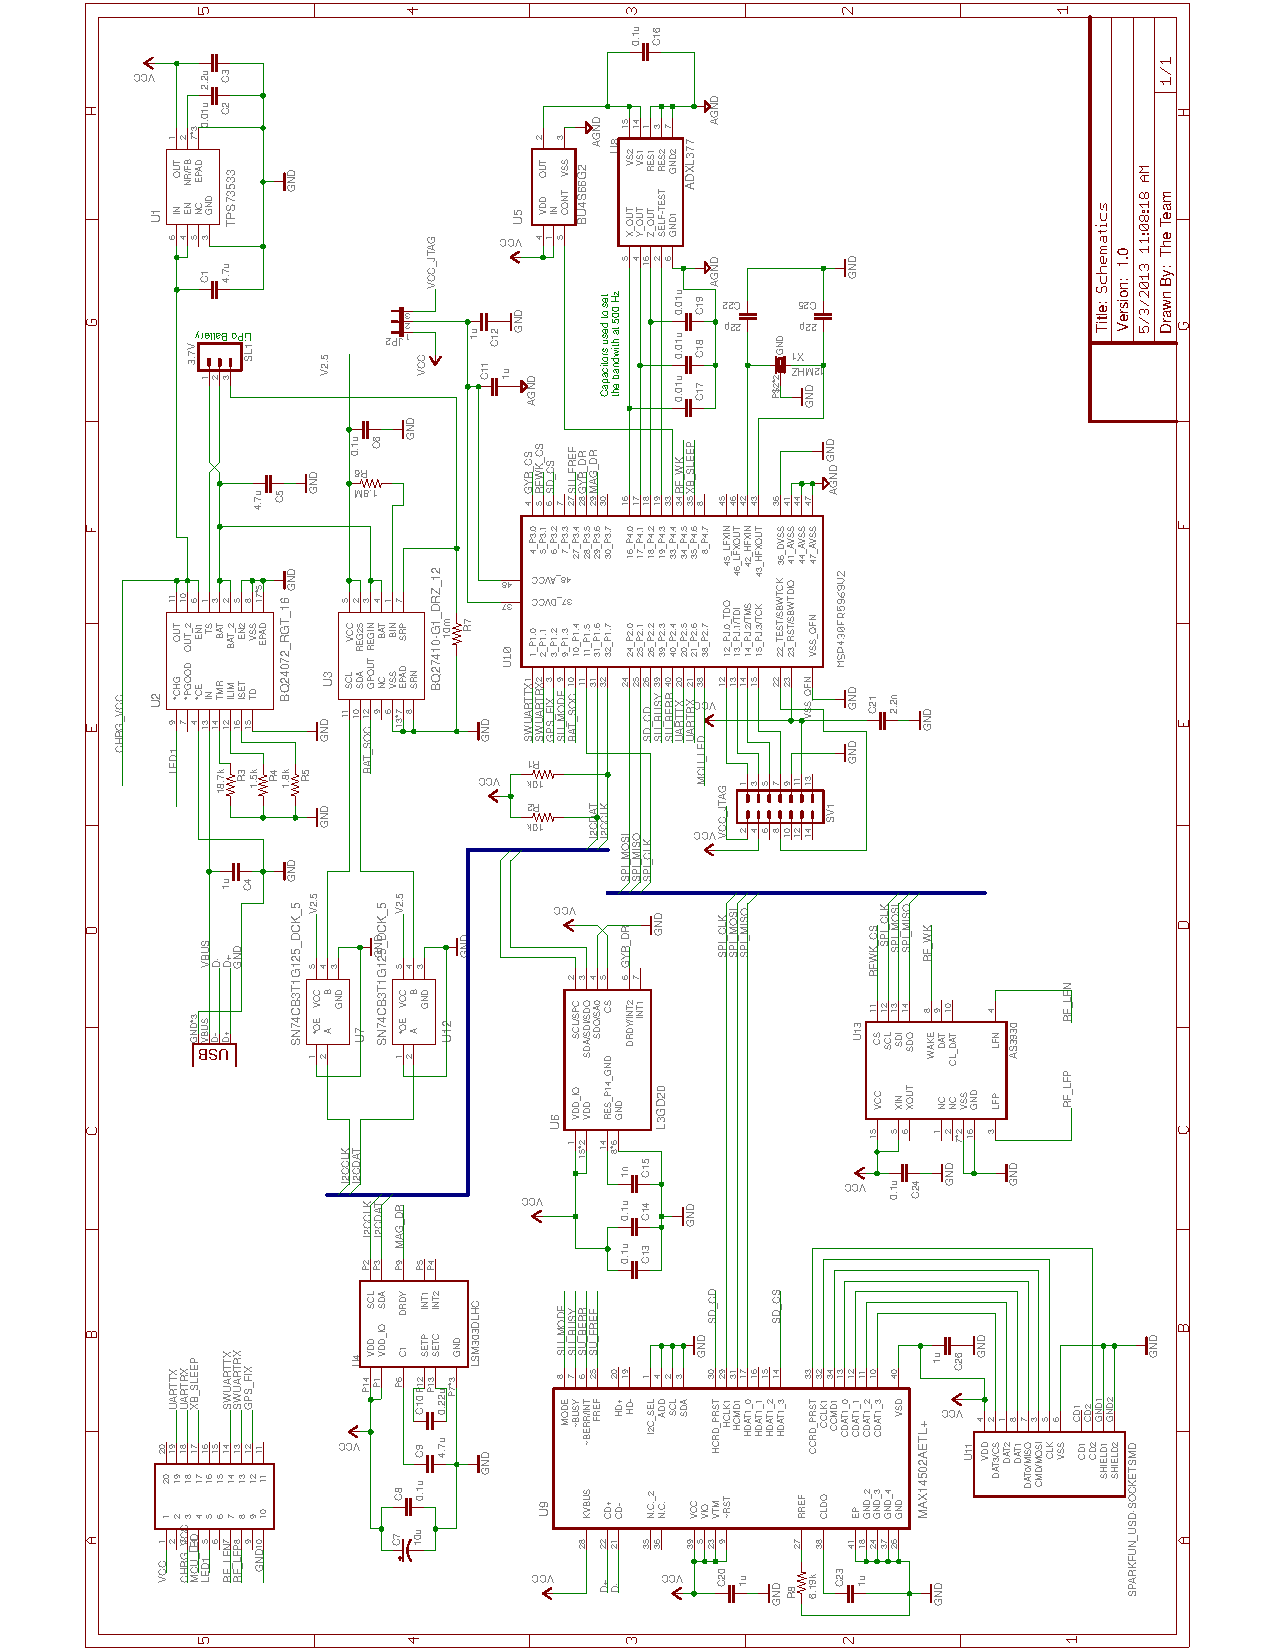
\includegraphics[width=0.95\textwidth]{img/1stLvlSchem}
	\caption{Schematic for First Level of PCB \label{fig:1stLvlSchem}}
\end{figure}

\begin{figure}[H]
	\centering
	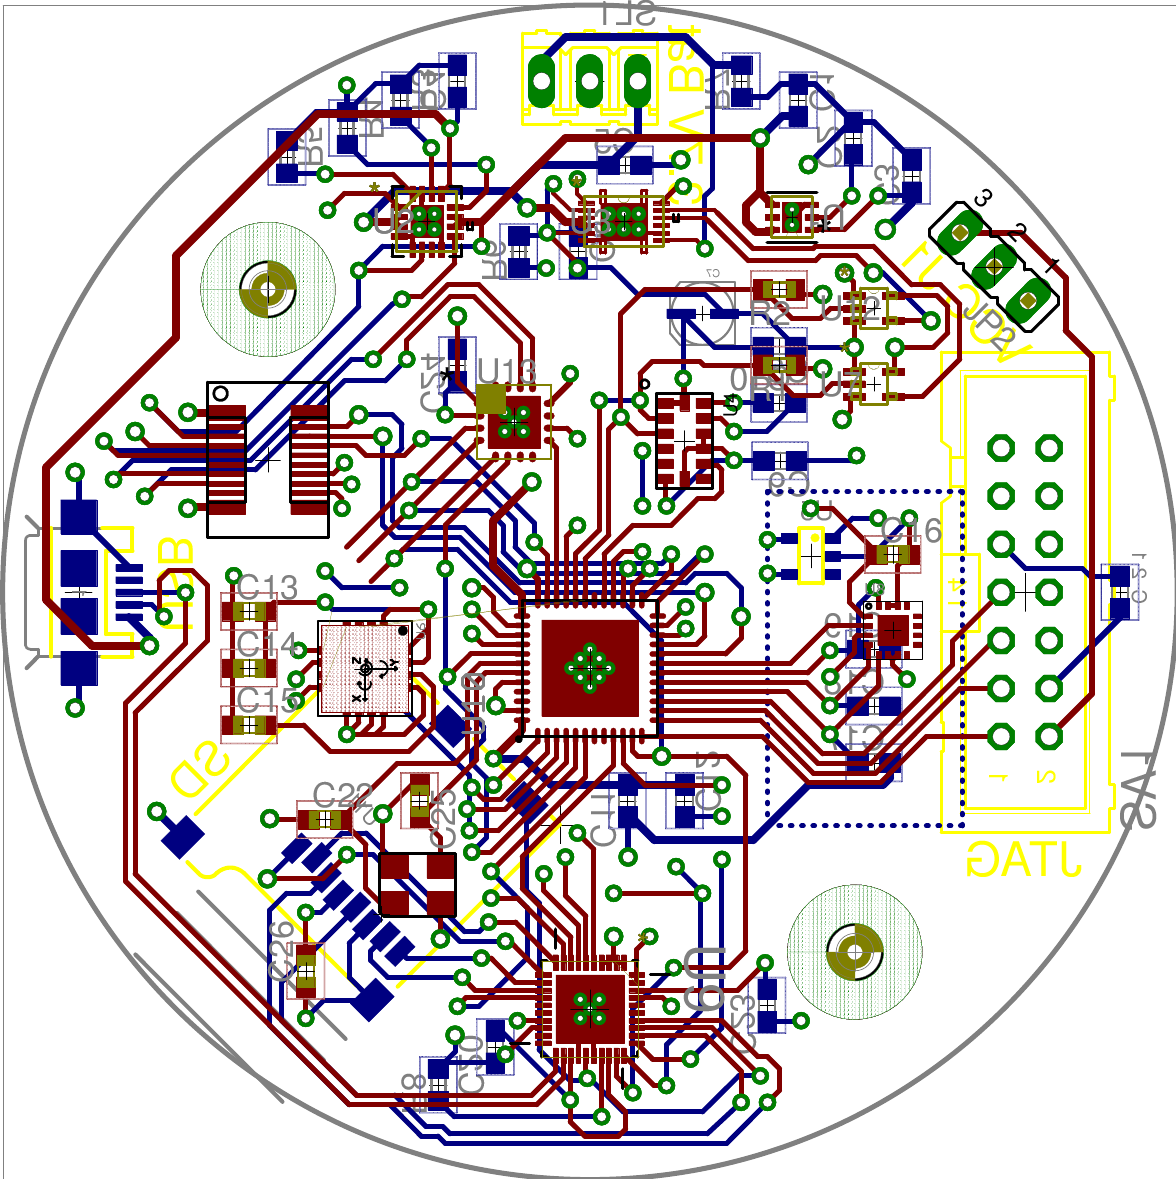
\includegraphics[width=0.95\textwidth]{img/1stLvlBoard.png}
	\caption{Schematic for First Level of PCB \label{fig:1stLvlBoard}}
\end{figure}

\begin{figure}[H]
	\centering
	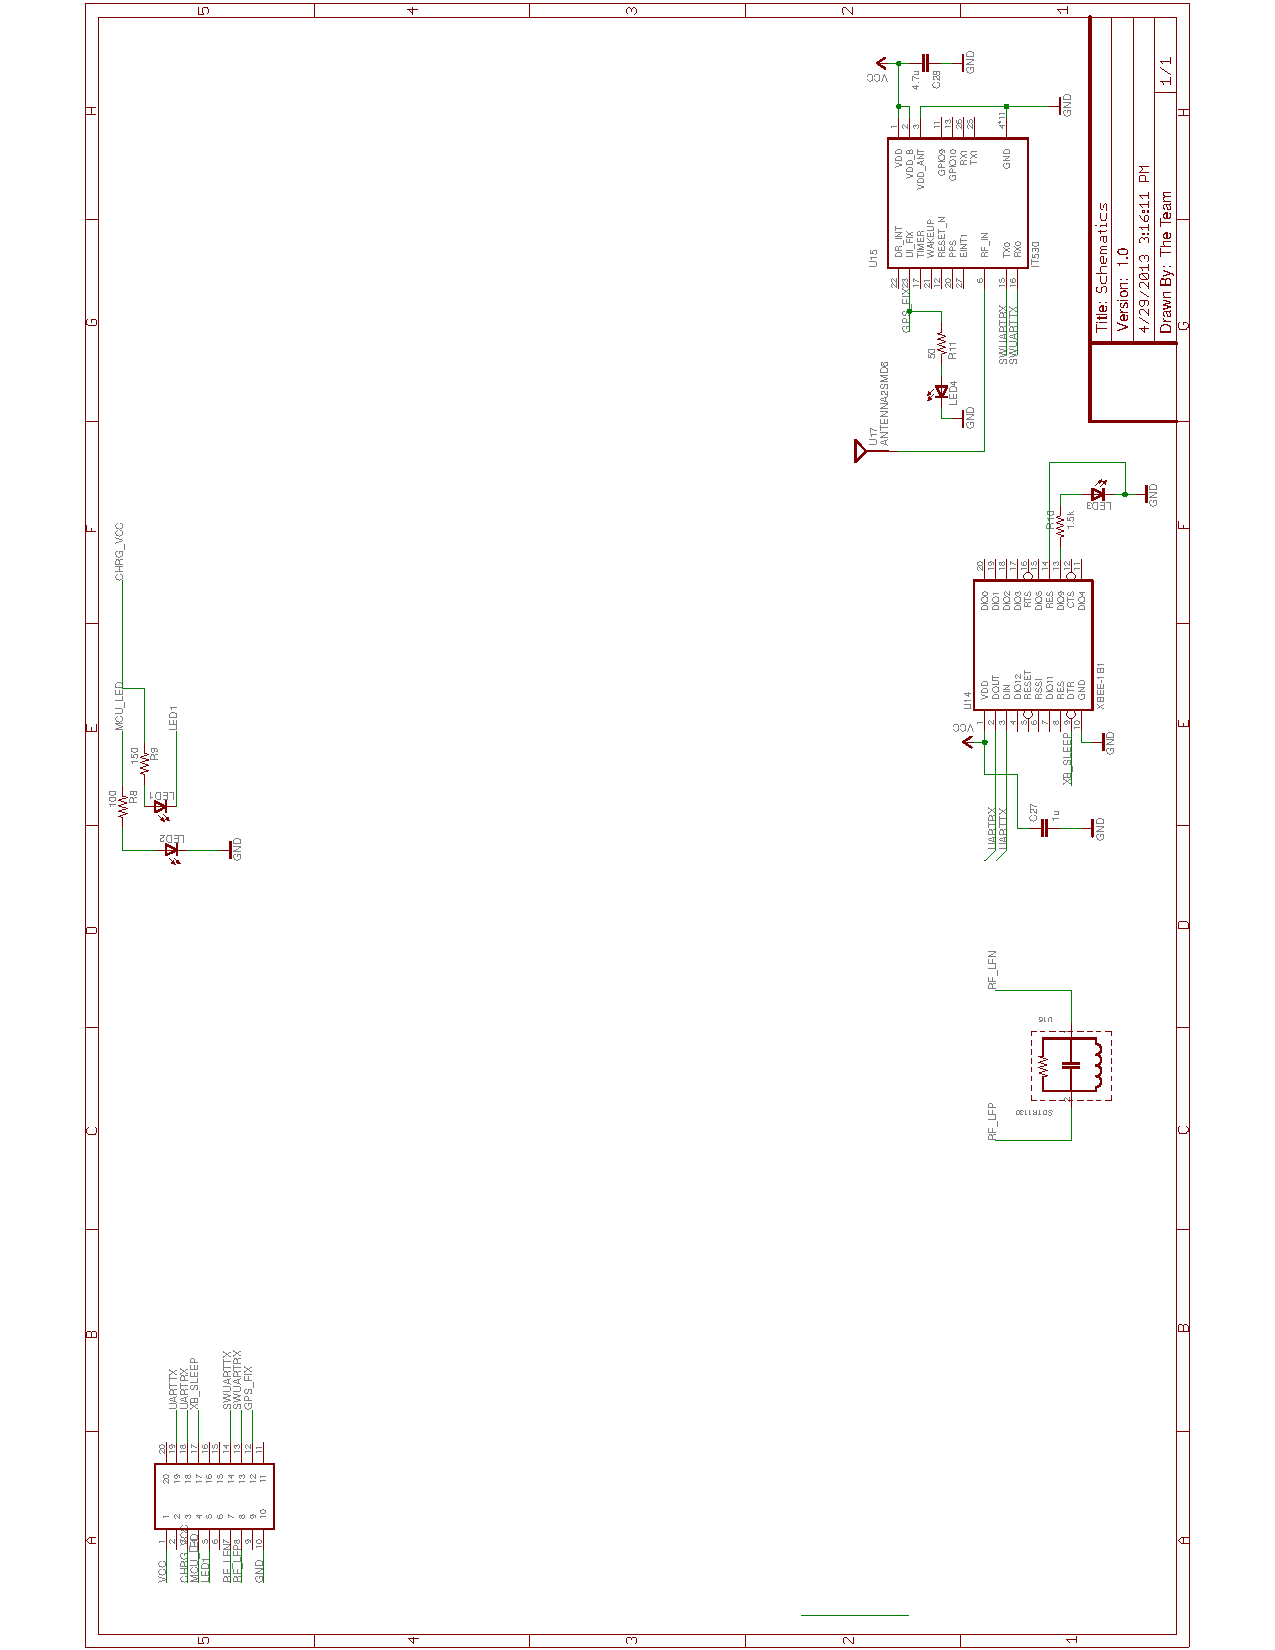
\includegraphics[width=0.95\textwidth]{img/2ndLvlSchem}
	\caption{Schematic for First Level of PCB \label{fig:2ndLvlSchem}}
\end{figure}

\begin{figure}[H]
	\centering
	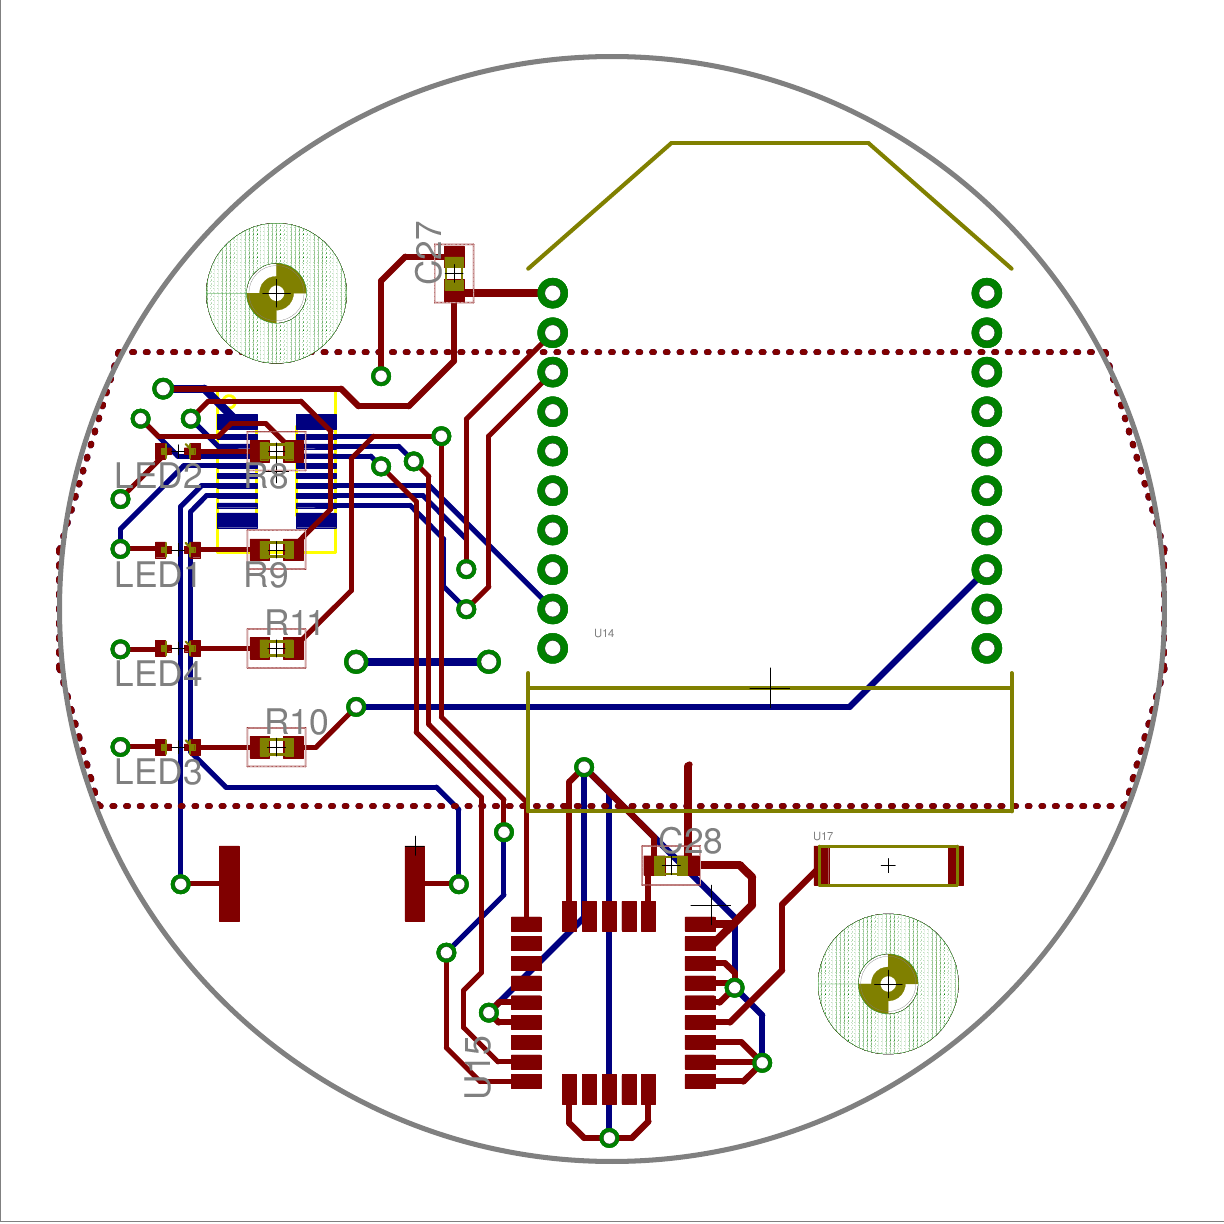
\includegraphics[width=0.95\textwidth]{img/2ndLvlBoard.png}
	\caption{Schematic for First Level of PCB \label{fig:2ndLvlBoard}}
\end{figure}